%Report
\documentclass[14pt]{extreport}
\usepackage{color}
\usepackage[cache=false]{minted}
\usepackage{afterpage}
\usepackage{graphicx}

% Command for inserting blank page
\newcommand\blankpage{
    \null
    \thispagestyle{empty}
    %\addtocounter{page}{-1}
    \newpage
    }

\title{High Performance Graph Processing in Partitioned Global Address Space Model}
\date{2020--12--10}
\author{Vahag Bejanyan}

\begin{document}
\maketitle
\pagenumbering{gobble}
\newpage
\pagenumbering{arabic}

\tableofcontents
\blankpage

\section{Introduction}
Graphs are playing an emerging role in the field of Computer Science. Various problems can be modeled and studied as graphs. Hence, to be able to solve large graph problems in an effective manner the fast, stable and accurate algorithms, new computation models and frameworks are needed to express graph-based computations and simulations. Often graphs can reach up to hundreds of million of vertices in size, hence a simple serial implementations are not feasible for such cases and parallel and distributed algorithms are needed. One of the widely used and adopted models to express distributed computations is Message Passing Interface(hereafter MPI) protocol. In essence, MPI provides an generic API through which various computation nodes can be grouped into communicator groups and exchange messages through both syncrhonous and asyncrhonous interfaces. Partitioned Global Address Space(hereafter PGAS) models act as an new alternative for distributed scalable computing. In a future sections of this document various PGAS powered models such as Chapel and UPC++ will be described. An overview of a actual research related to PGAS powered graph algorithms and models will be given. After this, research objectives will be sited alongside the action plan.

\blankpage

\section{Models, algorithms and frameworks}
\subsection{Overview of Parallel Programming Models}
\subsubsection{Shared Memory Models}
This model is based on a shared memory systems, where each memory location is accessiable by every computation node. Usually multithreaded programming models are implemented as a shared memory systems. In this model any memory location is globally accessible and control is syncrhonized through the usual syncrhonization primitives like mutexes. Many languages like C++11 provides an Abstract Memory Model which alongside with it's standardized threads support be used in shared memory system programming. Another examples are Pthreads and OpenMP which both provide API for multithreaded exectuion in shared memory systems.
\subsubsection{Distributed Memory Models}
In this model each processor maintains it's own local memory and knows nothing about other computation units.
To be able communicate in this model an message passing protocol(like MPI) should be established. For distributed memory model computing MPI provides rich set of features such as:
\begin{enumerate}
\item Point-to-point Two-sided Communication
\item Collective Communication 
\item One-Sided Communication
\item Job Startup
\item Parallel I/O
\end{enumerate}

\subsection{Partitioned Global Address Space}
Partitioned Global Address Space (PGAS) is a parallel programming model which assumes global view on address space which is partitioned within different processes. Below given a list of characteristics that language should specify to be considered as PGAS lanauge.
\begin{enumerate}
	\item It should specify a parallel execution model,
	\item It should provide a way to specify how a global address space should be partitioned,
	\item It should provide a way to describe how data is distributed over different partitions,
	\item Language should allow access to both shared and distributed data using shared-memory semantics.
\end{enumerate}

\paragraph{Parallel Execution Model}
This model describes detailes of launching and executing parallel activities(hereafter threads). PGAS model provides three main kinds of such activities.

\subparagraph{Single Program Multiple Data}
In this model at the program startup a fixed number of threads is created. Each thread has it's unique thread index and hence using this index, for example, it's possible to specify which data current thread should process.

\subparagraph{Asynchronous PGAS}
In this model at the program startup only one thread is created. Creation of a new threads has dynamic fashion and expressed using language specific constructs like \mintinline{chapel}{cobegin} in case of Chapel.

\subparagraph{Impilicit Parallelism} In this model no explicit parallelism is exists in code. Instead of that new thread creation is done by the language runtime and data distributed handled in an opaque way. Chapels \mintinline{chapel}{forall} construct is a good example of this concept. 

\subparagraph{Places Model}
Large-scale systems with multiple computational nodes often incorporate NUMA characteristics. To cope with this, in PGAS model global address space is partitioned into so called \textit{places}. This differentiation allows to easly express a affinity of a memory to it's computation node. This allows node to access memory with a minimal cost. On the other side, access to data from a different \textit{places} has higher cost.

\subparagraph{Data Distribution Model}\label{DataDistributionModelSubParagraph}
This model describes how data is distributed over different places. Distributions can be regular and irregular. An example of a regular distribution are globally distributed partitioned arrays which Chapel provied. Before creating such array an index set is specified which determines how data should be distributed over places(or \textit{Locales}) in case of Chapel). Several patterns are possible for regular distributions. For example (a) cyclic-distribution, (b) block-cyclic-distribution and (c) block-distribution are common.

\begin{figure}[H]
	\centering
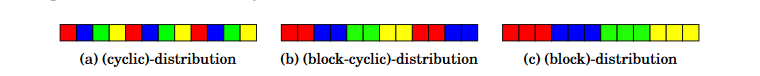
\includegraphics[scale=0.75]{distributions.png}
\end{figure}


Below given examples of how index set distribution can be expressed uing Chapel. 

\begin{listing}[H]
\begin{minted}[tabsize=4,linenos]{chapel}
// Make the program size configurable from the command line.
config const n = 8;

// Declare a 2-dimensional domain Space that we 
// will later use to initialize the distributed domains.
const Space = {1..n, 1..n};

// The Block distribution distributes a bounding 
// box from n-dimensional space across the target locale 
// array viewed as an n-dimensional virtual locale grid. 
// The bounding box is blocked into roughly equal 
// portions across the locales. 
// Note that domains declared over a Block distribution can also 
// store indices outside of the bounding box;
// the bounding box is merely used to compute the blocking of space.
const BlockSpace = Space dmapped Block(boundingBox=Space);
var BA: [BlockSpace] int;

// Cyclic distributions start at a designated n-dimensional 
// index and distribute the n-dimensional space across 
// an n-dimensional array of locales in 
// a round-robin fashion (in each dimension).
const CyclicSpace = Space dmapped Cyclic(startIdx=Space.low);
var CA: [CyclicSpace] int;

// Block-Cyclic distributions also deal out indices in a 
// round-robin fashion, but rather than dealing out 
// singleton indices, they deal out blocks of indices. 
// Thus, the BlockCyclic distribution is parameterized by 
// a starting index (as with Cyclic) and a block 
// size (per dimension) specifying how large the 
// chunks to be dealt out are.
const BlkCycSpace = Space dmapped BlockCyclic(startIdx=Space.low,
                                              blocksize=(2, 3));
var BCA: [BlkCycSpace] int;
\end{minted}
\caption{Examples of Index Distributions in Chapel}
\end{listing}

On the other side, irregular distribution can play a significant role in a construction of irregular data structures such as trees or hashmaps. UPC++(PGAS implementation for C++) achieves this in terms for \textit{Global Pointers}. Below given an example implementation of distributed hashmap using UPC++ and C++.

\begin{listing}[H]
\begin{minted}[tabsize=4,linenos]{c++}
class DistrMap {
	using dobj_map_t = upcxx::dist_object<
								std::unordered_map<std::string,	
												   std::string>>;
	dobj_map_t local_map;

	int get_target_rank(const std::string& key) {
		return std::hash<std::string>{}(key) % upcxx::rank_n();
	}

	public:
	DistrMap() : local_map({}) {}

	upcxx::future<> insert(const std::string& key, 
						   const std::string& val) {
		return upcxx::rpc(get_target_rank(key),
				[](dobj_map_t& lmap, 
				   const std::string& key, 
				   const std::string& val) {
				lmap->insert({key, val});
				}, local_map, key, val);
	}

	upcxx::future<std::string> find(const std::string& key) {
		return upcxx::rpc(get_target_rank(key),
				[](dobj_map_t& lmap, 
				   const std::string& key) -> std::string {
				auto elem = lmap->find(key);
				if (elem == lmap->end()) return std::string();
				return elem->second;
				}, local_map, key);
	}
};
\end{minted}
\caption{Distributed Hash Table using UPC++ Global Pointers}
\end{listing}

However, current PGAS models dosen't provide any standard irregular distributions like in case of regular ones in this should be done explicitly by sharing pointers.

\blankpage

\subparagraph{Data Access Model}
This model is tightly connected to the \ref{DataDistributionModelSubParagraph} as it's describes how data is distributed accross places, represented, declared and accessed. For example, in case of regular distributions a concept of local and glbal indexes is presented. Also an distinction in global data access syntax is present, then such access is called explicit.

\section{Research objectives}
\blankpage

\section{Related work}
\blankpage

\section{What has been done}
\blankpage

\section{Action plan}
\blankpage

\section{Articles and books}

\end{document}
